% !TEX root = ../mat999.tex
\newpage
\section{Lebesgue's integral}
Let $(\Omega, \F, \mu)$ be a measurable space, let $S^+$ denote the set of simple and non-negative $f: \Omega \mapsto \R^+$ defined by
\begin{equation*}
    f(\omega) = \bigs{k=1}^n \alpha_i \I_{A_i} (\omega)
\end{equation*}where $\alpha_i \in \bar{\R}^+$ and $A_i \in \F$ disjoint (if not, we can make it disjoint)

\begin{ex}[$f$ is measurable $(\Omega, \F) \mapsto (\bar{R}, \bar{B})$]
\end{ex}
\vspace{2cm}
\begin{dfn}{The Lebesgue Integral}
\begin{enumerate}
    \item if $f \in S^+$ then 
    \begin{equation*}
        \int f(\omega) d\mu(\omega) = \int_{\Omega} f d\mu := \bigs{i=1}^n \alpha_i \mu(A_i)
    \end{equation*}
    \item if $f: \Omega \mapsto (\bar{R}^+, \bar{\B})$ is measurable and non-negative then the integral of $f$ w.r.t $\mu$ is 
    \begin{equation*}
        \int_{\Omega} f d\mu := \supunder{h\leq f, h\in S^+} \int h d\mu
    \end{equation*}
    \textbf{Remark: Since we allow the value of $\infty$, we define $0 \cdot \infty :=0$}
\end{enumerate}
\end{dfn}
\begin{ex}
Check that $\int_{\Omega} f d\mu$ is well defined.\\
(if we partition $\Omega$ in different ways, will we get same value back ?) \\
\end{ex}
\begin{ex}
Check that for $f\in S^+$ both definition (1,2) agree
\end{ex}
\newpage
\begin{thm}[Properties of Lebesgue's integral]
Let $f,g: X \mapsto (\bar{R}^+, \bar{\B})$ be measurable, non-negative functions 
\begin{enumerate}
    \item if $f\leq g$ then $\int f d\mu \leq \int g d\mu$
    \item $c\geq 0 \int cf d\mu = c\int fd\mu$
    \item if $A,B\in \F$ and $A\subset B$ then \begin{equation*}
        \int_A fd\mu \leq \int_B fd\mu \text{ where } \int_A fd\mu := \int_\Omega f \I_A d\mu 
    \end{equation*}
    \item $A\in \F$, then $\int_A fd\mu = 0$ iff $f=0$ a.e on $A$, i.e. $\mu\{\{f>0\} \cap A\} = 0$
    \item if $f, g\geq 0$ then $\int_\Omega (f+g) d\mu = \int_\Omega f d\mu+\int_\Omega g d\mu$
\end{enumerate}
\end{thm}
\pf 
\newpage
\begin{lem}[Approximating function by simple functions] Let $f$ be measurable non-negative function then $\exists (g_n) \subset S^+$ s.t. $g_n(\omega)\uparrow f(\omega)$ as $n \rightarrow \infty$ for any $\omega\in \Omega$
\end{lem}
\pf Construction:\begin{equation*}
    g_n := \bigs{k=1}^{n2^n} \frac{k-1}{2^n} \I_{\{\frac{k-1}{2^n} \leq f\leq \frac{k}{2^n\}}} + n \I_{\{f\geq n\}} 
\end{equation*}Then $g_n\in S^+$, fix $\omega \in \Omega$:
\begin{enumerate}
    \item if $f$ is bounded, $f(\omega) < n $ then $0 \leq f(\omega) - g_n(\omega)\leq \frac{1}{2^n}$
    \item if $f$ is unbounded, $f(\omega) = \infty $(unbounded), then $g_n(\omega) \rightarrow \infty$
\end{enumerate}
 In both case $g(\omega)\xrightarrow{n\rightarrow \infty} f(\omega)$ for any $\omega\in \Omega$

\begin{thm}[Monotone Convergence Theorem(MCT)]\label{MCT} let $f_n$ be non-decreasing of non-negative measurable functions, and $f_n(\omega)\uparrow f(\omega)$ as $n \rightarrow \infty$. Then 
\begin{equation*}
    \biglim{n\rightarrow \infty} \int_\Omega f_n d\mu = \int_\Omega f d\mu
\end{equation*}
\end{thm}
\pf From property (1) of integrals (monotonicity) of integrals:
\begin{equation*}
    \int_\Omega f_n d\mu \leq \int_\Omega f d\mu \quad \left( \int_\Omega f_nd\mu \right) \text{ is non decreasing}
\end{equation*}
Note: The limits of bounded monotonic sequence exist \\
It is enough to show
\begin{equation*}
    \biglim{n\rightarrow \infty} \int_\Omega f_n d\mu \leq \int_\Omega f d\mu
\end{equation*}Let $g \in S^+, g\leq f$. Fix $t\in (0,1)$ Then $A_n:= \{\omega | f_n(\omega) \geq tg(\omega)$ is an increasing measurable sets and $\bigu{n}A_n = \Omega$
\begin{equation*}
    \int_{\Omega} f_n(\omega) \geq \int_{A_n} f_n(\omega) d\mu \geq t \int_{A_n} g(\omega) d\mu
\end{equation*}Represent $g = \bigs{k=1}^{N} \alpha_k \I_{E_k}$ then 
\begin{equation*}
    \int_{A_n} g(\omega) d\mu = \int_{\Omega} \bigs{k=1}^{N} \alpha_k \I_{E_k \cap A_n}(\omega) d\mu =  \bigs{k=1}^{N} \alpha_k \mu(E_k \cap A_n) = \bigs{k=1}^{N} \alpha_k \mu(E_k) = \int_{\Omega} g(\omega) d\mu
\end{equation*}Since $A_n$ is increasing and we have continuity of measure from below we have $\mu(E_k \cap A_n) \rightarrow \mu(E_k)$ as $n \rightarrow \infty$ for all $k$ \\
Recall we have
\begin{align*}
    \int_{\Omega} f_n(\omega) &\geq \int_{A_n} f_n(\omega) d\mu \geq t \int_{A_n} g(\omega) d\mu \rightarrow t \int_{\Omega} g(\omega) d\mu \quad \forall t \in (0,1) \\
    &\text{This is true for all $t\in(0,1)$ Take $t \rightarrow 1$} \\
    \int_{\Omega} f_n(\omega) &\geq \int_{\Omega} g(\omega) d\mu \quad \forall g \in S^+, g \leq f \\
    \Rightarrow \int_{\Omega} f_n(\omega) &\geq \supunder{g\leq f, g\in S^+} \int_{\Omega} gd\mu = \int_{\Omega} fd\mu
\end{align*}
\qed
\newpage
\begin{example}
[Things might go wrong if $f_n$ is not "non-decreasing"]let $(\Omega, \F, \prob) = ((0,1), \B, \lambda)$ and $f_n:= n\I_{0,\frac{1}{n}}$.
\begin{align*}
    &\int_\Omega f_n d\mu = n \cdot \lambda((0,\frac{1}{n})) = 1 \quad n\in \N\\
    &f_n \xrightarrow{n\rightarrow \infty} 0\quad \forall \omega \in (0,1) \\
    \biglim{n\rightarrow \infty}& \int_\Omega f_n d\mu = 1 \neq \int_\Omega 0 d\mu =0
\end{align*}For example, for $\omega = \frac{3}{4}, f_1(\omega)=1, f_2(\omega)=0$ which is decreasing, does not satisfy MCT conditions.\\[0.5cm]
But this satisfies condition of Fatou's lemma \ref{Fatou}. \\
$f_n \rightarrow 0, \linf{n}f_n =0, \into f_n d\mu = 1 \rightarrow \linf{n}\into f_n d\mu = 1$
\begin{equation*}
    \into \linf{n}f_n \diff \mu =0 \leq \linf{n}\into f_n \diff\mu =1
\end{equation*}
\end{example}

\begin{ex}If $f, g\geq 0$ then $\int_\Omega (f+g) d\mu = \int_\Omega f d\mu+\int_\Omega g d\mu$
\end{ex}
\newpage
\begin{thm}[Fatou's Lemma]\label{Fatou}
let $f_n$ be sequence of measurable non negative functions, then 
\begin{equation*}
    \into \linf{n} f_n d\mu \leq \linf{n}\into f_n d\mu
\end{equation*}
\end{thm}
\pf let $g_n := \infunder{k\geq n}f_k$ This is non decreasing, and measurable sequence. \\
$g_n \leq f_n$ and $g_n \uparrow \linf{n}f_n$.
\begin{align*}
    &\biglim{n\rightarrow\infty}\into g_n d\mu = \into \linf{n}f_n d\mu \\
    &\biglim{n\rightarrow\infty}\into g_n d\mu = \linf{n}\into g_n d\mu \leq \linf{n}\into f_n d\mu \text{ by MCT and monotonicity}\\
    \Rightarrow& \into \linf{n}f_n d\mu \leq \linf{n}\into f_n d\mu
\end{align*}
\qed
\begin{ex}[Reverse Fatou's Lemma]
let $f_n$ be sequence of measurable non negative functions s.t, $f_n\leq g$ for some measurable $g$ with $\int g d\mu < \infty$ then 
\begin{equation*}
    \int_{\Omega} \lsup{n} f_n d\mu \geq \lsup{n}\int_{\Omega} f_n d\mu
\end{equation*}
\end{ex}
\newpage
\begin{dfn}
For $f: \Omega \mapsto (\bar{\R}, \bar{\B})$ measurable, we define:
\begin{enumerate}
    \item $f^+ :=\max(f, 0) \geq 0$
    \item $f^- :=\max(-f, 0) = -\min(f, 0) \geq 0$
\end{enumerate}
\end{dfn}
observe: $f = f^+ - f^-$ and $\abs{f} = f^+ + f^-$, $f$ is measurable iff $f^+, f^-$ are both measurable.

\begin{dfn}[Lebesgue integral for measurable functions]
If $f: \Omega \mapsto (\bar{\R}, \bar{\B})$ measurable, we define:
\begin{equation*}
    \into fd\mu := \into f^+ d\mu -\into f^- d\mu
\end{equation*}provided that at least one of the integrals on the RHS is finite, otherwise $(\infty-\infty)$ is problematic
\end{dfn}
\textbf{Now we have all three definitions of Lebesgue integral.}
\vspace{0.5cm}
\begin{dfn}[Integrable] we say $f$ is integrable if
\begin{equation*}
    \text{both }\into f^+ d\mu,\into f^- d\mu \text{ are finite } \Longleftrightarrow \into |f|d\mu < \infty
\end{equation*}
\end{dfn}
\begin{thm}[Properties]Let $f,g$ are integrable
\begin{enumerate}
    \item $f+g$ is integrable and $\int f+g d\mu = \int f d\mu +\int g d\mu$
    \item If $c\in\R$ then $\int cf d\mu = c\int f d\mu$ \\
    (Combing 1 and 2 we have $\int \alpha f+ \beta g d\mu = \alpha\int f d\mu +\beta\int g d\mu \quad \forall \alpha,\beta \in \R$)
    \item if $f\leq g$ then, $\int f d\mu \leq \int g d\mu$
    \item $|\int_{\Omega} f d\mu| \leq \int_{\Omega} |f| d\mu$
    \item If $A_n\in \F$ disjoint, $\bigu{n}A_n = \Omega$ then
    \begin{equation*}
        \into f d\mu = \bigs{n} \int_{A_n} f d\mu
    \end{equation*}
    \item If $\int_{A} f d\mu=0 \quad \forall A\in \F$ iff $f = 0$ a.e.
\end{enumerate}
\end{thm}
\newpage
\begin{cor}\label{equalint}
If $f$ and $g$ are measurable and $f = g$ a.e. then $f$ is integrable iff $g$ is integrable and 
\begin{equation*}
    \int f d\mu = \int g d\mu
\end{equation*}
\end{cor}

\begin{cor}[Fatou's Lemma in more general sense]
let $f_n$ be sequence of measurable functions with $f_n \geq 0$ a.e., then 
\begin{equation*}
    \into \linf{n} f_n d\mu \leq \linf{n}\into f_n d\mu
\end{equation*}
\end{cor}

\begin{cor}[MCT in more general sense]
let $f_n$ be non-decreasing of non-negative measurable functions, and $f_n(\omega)\uparrow f(\omega)$ a.e Then 
\begin{equation*}
    \biglim{n\rightarrow \infty} \int_\Omega f_n d\mu = \int_\Omega f d\mu
\end{equation*}
\end{cor}
\vspace{2cm}
\pf Let $g_n = \max(f_n, 0)$, then $g_n \in \F^+$ (max of measurable function is measurable and it is also non negative). Let $N = \{\omega| g_n \neq f_n\}$ observe that:
\begin{equation*}
    N = \{\omega| g_n \neq f_n\} = \{\omega| \max(f_n, 0) \neq f_n\} = \{\omega| f_n < 0\}
\end{equation*}$\mu(\{f_n< 0\}) = 0$ since $f_n \geq 0$ a.e., $\mu(N) = 0$. Hence $g_n = f_n$ a.e. and hence
\begin{equation*}
    \linf{n} g_n = \linf{n} f_n \quad \text{a.e.}
\end{equation*}
By Corollary \ref{equalint} and Fatou's Lemma (Assume we have integrability): 
\begin{equation*}
    \int \linf{n}f_n d\mu = \int \linf{n}g_n d\mu \leq  \linf{n}\int g_n d\mu = \linf{n}\int f_n d\mu
\end{equation*}
\newpage
\subsection*{Riemann Integral}
\begin{figure}[h]
    \centering
    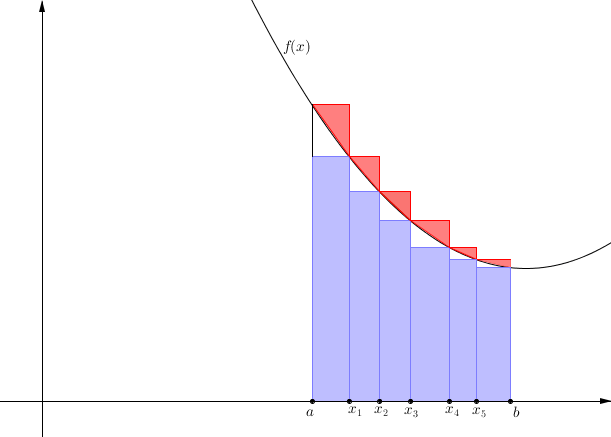
\includegraphics[scale = 0.5]{integral.png}
    \caption{Upper and Lower Riemann sums}
    \label{fig:my_label}
\end{figure}
Consider function $f:[a,b] \mapsto \R$ \\
We partition $[a,b], \setp := \{a_i\}_{i=1}^k$ s.t. $a = a_0 < a_1 < ... < a_k = b$ \\
Define:
\begin{itemize}
    \item $m_i := \inf\{f(x)| x\in [a_{i-1},a_i]\}$
    \item $M_i := \sup\{f(x)| x\in [a_{i-1},a_i]\}$
    \vspace{0.5cm}
    \item Lower sum corresponding to partition $\setp \quad L(f,\setp):= \bigs{i=1}^k m_i (a_i - a_{i-1})$
    \item Upper sum corresponding to partition $\setp \quad  U(f,\setp):= \bigs{i=1}^k M_i (a_i - a_{i-1})$
    \vspace{0.5cm}
    \item Lower Riemann integral $L(f):= \sup\{L(f,\setp): \setp \in \tilde{\setp}\}$
    \item Upper Riemann integral $U(f):= \inf\{U(f,\setp): \setp \in \tilde{\setp}\}$ \\
    $\tilde{\setp}$ be the  set of all possible partitions of $[a,b]$
\end{itemize}
\begin{dfn}[Riemann Integrable]
$f:[a,b] \mapsto \R$ is Riemann integrable if $L(f) = U(f)$. In that case we define the integral of $f$ by
\begin{equation*}
    \int_a^b f(x) dx = I = U(f) = L(f)
\end{equation*}
\end{dfn}
\newpage
\subsubsection*{Connections between Riemann and Lebesgue integral}Suppose we have a Riemann integrable function $f$, \textcolor{blue}{WTS: This function is also Lebesgue integrable, first it has to be measurable} \\
Suppose $f:[a,b] \mapsto \R^+$ is Riemann integrable with $\int_a^b f(x) dx = I$ Then there exists sequence $l_n, u_n \in S^+$ s.t.
\begin{enumerate}
    \item $l_n \uparrow l \leq f$ and $u_n \downarrow u \geq f$
    \item For $u_n, l_n\in S^+$ the Lebesgue integral is defined equal to Riemann integrals $\int l_n d\lambda = \int_a^b l_n dx$. 
    \begin{equation*}
        L(f,\setp_n) = \int_a^b l_n dx \uparrow L \Rightarrow \int l_n d\lambda \uparrow L
    \end{equation*} Similarly, $\int u_n d\lambda \downarrow U$
\end{enumerate}Hence $l$ and $u$ are both measurable (limit of measurable functions are measurable) with $l \leq u$ and 
\begin{equation*}
    \int l_n d\lambda \leq \int l d\lambda \leq \int u d\lambda \leq \int u_n d\lambda 
\end{equation*} And by MCT, we have
\begin{align*}
    &\int l_n d\lambda \rightarrow \int l d\lambda, \int u_n d\lambda \rightarrow \int u d\lambda \\
    &\int l_n d\lambda \rightarrow I, \int u_n d\lambda \rightarrow I
\end{align*} We have, by additivity:
\begin{align*}
    \int l d\lambda +&\int (u-l) d\lambda = \int u d\lambda \\ 
    &\int (u-l) d\lambda = 0
\end{align*}We also know that $u-l$ is positive and measurable (difference of limits of measurable function), by property 4 we have $u = l$ a.e. \hfill (*)
\begin{align*}
    &l_n \leq f \leq u_n \text{ for any n} \\
    & l_n \uparrow l, u_n\downarrow u \\
    \Rightarrow& l \leq f \leq u \\
    &u = f = l \text{ on } \{u=l\} (a.e.) \qquad(*)
\end{align*}Denote $\tilde{f} = f \I_{\{u=l\}} = uI_{\{u=l\}}$ which is measurable (product of two measurable functions) \\
and $f = \tilde{f} + f\I_{\{u\neq l\}}$
\begin{ex}
Show that with $\setl = $Lebesgue (completion of Borel $\sigma$-algebra w.r.t $\lambda$)
\begin{equation*}
    f([a,b], \setl, \lambda) \mapsto (\R, \B)
\end{equation*} is measurable.
\end{ex}
\begin{cor}$f$ is Lebesgue $([a,b], \setl, \lambda)$ integrable and $\int f d\lambda = I$
\end{cor}
\vfill
\textbf{Comments: This allows us to compute Lebesgue integral $\int fd\lambda$ using The Fundamental Theorem of Calculus for Riemann integrable function.}
\begin{example}
$(\Omega, \F, \mu) = ([0,1], \B, \lambda)$ Let $f_n(x) = (n+1)x^n$ then
\begin{equation*}
    \int f_n d\lambda = \int_0^1 f_n(x) dx = x^{n+1} \Big\rvert_0^1 = 1
\end{equation*}
\end{example}